\documentclass[11pt,a4paper]{article}
\usepackage{cmap}
\usepackage[T1]{fontenc}
\usepackage[utf8]{inputenc}
\usepackage[romanian]{babel}
\usepackage{lmodern}
\usepackage[margin=22mm]{geometry}
\usepackage{amsmath,amssymb,graphicx,booktabs,longtable,array}
\usepackage{xcolor,listings,microtype,enumitem,fancyhdr}
\usepackage{tikz}
\usepackage[unicode,hidelinks,breaklinks]{hyperref}
\definecolor{accent}{HTML}{153F65}
\definecolor{codebg}{HTML}{F4F6F8}
\setlength{\parindent}{0pt}
\setlength{\parskip}{5pt}
\setlength{\emergencystretch}{3em}
\setlist[itemize]{leftmargin=*,nosep}
\pagestyle{fancy}\fancyhf{}
\fancyhead[L]{\small Testarea Sistemelor Software}
\fancyhead[R]{\small Documentație de laborator}
\fancyfoot[C]{\thepage}
\setlength{\headheight}{14pt}
\lstset{basicstyle=\ttfamily\scriptsize,breaklines=true,breakatwhitespace=false,
 columns=fullflexible,keepspaces=true,showstringspaces=false,
 backgroundcolor=\color{codebg},frame=single,rulecolor=\color{black!15},
 keywordstyle=\color{accent}\bfseries,commentstyle=\color{black!55},
 numbers=left,numberstyle=\tiny\color{black!45},numbersep=7pt,
 extendedchars=true,inputencoding=utf8,
 literate={ă}{{\u a}}1 {â}{{\^a}}1 {î}{{\^i}}1 {ș}{{\c s}}1 {ț}{{\c t}}1
 {Ă}{{\u A}}1 {Î}{{\^I}}1 {Ș}{{\c S}}1 {Ț}{{\c T}}1}
\hypersetup{pdftitle={Număr Armstrong de trei cifre},pdfauthor={},pdfsubject={EP, BVA, CEG, MC/DC și testare de mutație}}
\begin{document}
\begin{titlepage}
\centering
{\Large Testarea Sistemelor Software\par}
\vspace{22mm}
{\color{accent}\Huge\bfseries Număr Armstrong de trei cifre\par}
\vspace{10mm}
{\Large Proiect de laborator\par}
\vspace{6mm}
{\large Mihalache Sebastian-Stefan \textbf{506}\par}
{\large Neculae Andrei-Fabian \textbf{506}\par}
\vfill
\vspace{12mm}
{\large 4 noiembrie 2026\par}
\end{titlepage}
\section{Enunțul temei și criterii de acceptare}
Se dă un număr natural de exact trei cifre, 100 \ensuremath{\leq} n \ensuremath{\leq} 999.\allowbreak{} Să se determine dacă n este egal cu suma cuburilor cifrelor sale.\allowbreak{} Un asemenea număr se numește număr Armstrong de trei cifre.\allowbreak{}

Să se scrie un program care va afișa mesajul:
\begin{itemize}[label=\textendash]
\item \texttt{DA}, dacă numărul este egal cu suma cuburilor cifrelor sale
\item \texttt{NU}, dacă numărul este de trei cifre și diferă de suma cuburilor cifrelor sale
\item \texttt{INVALID}, dacă numărul este în afara intervalului închis [100,999]
\end{itemize}

\subsection{Exemple}

\begin{tabular}{@{}l@{\quad}c@{\quad}l@{}}
Pentru $n=153$, avem $1^{3}+5^{3}+3^{3}=1+125+27=153$
& $\Rightarrow$ & rezultatul este \textbf{DA}. \\[5pt]
Pentru $n=123$, avem $1^{3}+2^{3}+3^{3}=1+8+27=36$
& $\Rightarrow$ & rezultatul este \textbf{NU}.
\end{tabular}

\section{Partiționarea în clase de echivalență}
\textbf{Date de intrare:} $n$, număr întreg

\textbf{Clase intrări:}
\begin{itemize}[label=\textendash]
\item $N_1=\{n\mid 100\leq n\leq999\}$ intrări valide
\item $N_2=\{n\mid n<100\}$ intrări sub limita inferioară
\item $N_3=\{n\mid n>999\}$ intrări peste limita superioară
\end{itemize}

\textbf{Clase ieșiri:}
\begin{itemize}[label=\textendash]
\item $I_1$: \texttt{DA}, pentru un număr Armstrong de trei cifre
\item $I_2$: \texttt{NU}, pentru un număr din interval care nu este Armstrong
\item $I_3$: \texttt{INVALID}, pentru un număr în afara intervalului
\end{itemize}

\textbf{Clase de echivalență finale:}
\begin{itemize}[label=\textendash]
\item $C_1=\{n\in N_1\mid \text{ ieșirea }I_1\}$ $\Rightarrow$ test $n=153$
\item $C_2=\{n\in N_1\mid \text{ ieșirea }I_2\}$ $\Rightarrow$ test $n=123$
\item $C_3=\{n\in N_2\mid \text{ ieșirea }I_3\}$ $\Rightarrow$ test $n=99$
\item $C_4=\{n\in N_3\mid \text{ ieșirea }I_3\}$ $\Rightarrow$ test $n=1000$
\end{itemize}

\textbf{Teste:}
\begingroup\scriptsize\setlength{\tabcolsep}{2pt}
\begin{longtable}{@{}>{\raggedright\arraybackslash}p{0.3000\linewidth}>{\raggedright\arraybackslash}p{0.3000\linewidth}>{\raggedright\arraybackslash}p{0.3000\linewidth}@{}}
\toprule
\textbf{Test} & \textbf{n} & \textbf{Afișare program} \\

\midrule\endfirsthead
\toprule
Test & n & Afișare program \\

\midrule\endhead
\bottomrule\endfoot
EP01 & 153 & DA \\
EP02 & 123 & NU \\
EP03 & 99 & INVAL\allowbreak{}ID \\
EP04 & 1000 & INVAL\allowbreak{}ID \\

\end{longtable}
\endgroup

\begin{minipage}{\linewidth}
\textbf{Implementarea testelor și raportul de acoperire}
\begin{lstlisting}[language=Java,firstnumber=1]
public class EquivalncePartitioning {
    @Test
    public void EP01() {
        assertEquals("DA", Main.evaluate(153));
    }

    @Test
    public void EP02() {
        assertEquals("NU", Main.evaluate(123));
    }

    @Test
    public void EP03() {
        assertEquals("INVALID", Main.evaluate(99));
    }

    @Test
    public void EP04() {
        assertEquals("INVALID", Main.evaluate(1000));
    }

}
\end{lstlisting}

\textbf{Rezultatul execuției:} \texttt{OK (4 tests)}

\begin{center}
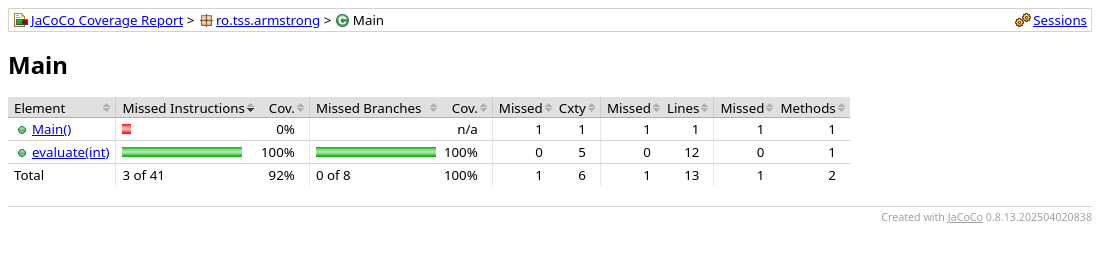
\includegraphics[width=\linewidth]{figuri/coverage_eptest_v02.png}
\par\small Raport JaCoCo pentru suita Equivalence partitioning
\end{center}
\end{minipage}




\section{Analiza valorilor de frontieră}
\textbf{Date de intrare:} $n$, număr întreg.

\textbf{Frontiere:} intervalul valid este $[100,999]$ \\ 
La limita inferioară alegem $n=\{99, 100, 101\}$ \\
La limita superioară alegem $n=\{998, 999, 1000\}$ \\
Astfel verificăm valorile imediat exterioare, limitele și vecinii interiori.

\textbf{Caz special:} numerele Armstrong de trei cifre sunt
$153,370,371,407$. Le verificăm împreună cu vecinii lor:
$152,153,154$; $369,370,371,372$; $406,407,408$.
Valorile $370$ și $371$ sunt consecutive și trebuie să producă ambele \texttt{DA}, prin urmare nu putem presupune că vecinul unui număr Armstrong produce automat \texttt{NU}.

\textbf{Teste:}

\begingroup\scriptsize\setlength{\tabcolsep}{2pt}
\begin{longtable}{@{}>{\raggedright\arraybackslash}p{0.3000\linewidth}>{\raggedright\arraybackslash}p{0.3000\linewidth}>{\raggedright\arraybackslash}p{0.3000\linewidth}@{}}
\toprule
\textbf{Test} & \textbf{n} & \textbf{Afișare program} \\

\midrule\endfirsthead
\toprule
Test & n & Afișare program \\

\midrule\endhead
\bottomrule\endfoot
BVA01 & 99 & INVAL\allowbreak{}ID \\
BVA02 & 100 & NU \\
BVA03 & 101 & NU \\
BVA04 & 152 & NU \\
BVA05 & 153 & DA \\
BVA06 & 154 & NU \\
BVA07 & 369 & NU \\
BVA08 & 370 & DA \\
BVA09 & 371 & DA \\
BVA10 & 372 & NU \\
BVA11 & 406 & NU \\
BVA12 & 407 & DA \\
BVA13 & 408 & NU \\
BVA14 & 998 & NU \\
BVA15 & 999 & NU \\
BVA16 & 1000 & INVAL\allowbreak{}ID \\

\end{longtable}
\endgroup

\textbf{Implementarea testelor și raportul de acoperire}
\begin{lstlisting}[language=Java,firstnumber=1,lineskip=-1pt]
public class BoundaryValueAnalysis {
    @Test
    public void BVA01() {
        assertEquals("INVALID", Main.evaluate(99));
    }

    @Test
    public void BVA02() {
        assertEquals("NU", Main.evaluate(100));
    }

    @Test
    public void BVA03() {
        assertEquals("NU", Main.evaluate(101));
    }

    @Test
    public void BVA04() {
        assertEquals("NU", Main.evaluate(152));
    }

    @Test
    public void BVA05() {
        assertEquals("DA", Main.evaluate(153));
    }

    @Test
    public void BVA06() {
        assertEquals("NU", Main.evaluate(154));
    }

    @Test
    public void BVA07() {
        assertEquals("NU", Main.evaluate(369));
    }

    @Test
    public void BVA08() {
        assertEquals("DA", Main.evaluate(370));
    }

    @Test
    public void BVA09() {
        assertEquals("DA", Main.evaluate(371));
    }

    @Test
    public void BVA10() {
        assertEquals("NU", Main.evaluate(372));
    }

    @Test
    public void BVA11() {
        assertEquals("NU", Main.evaluate(406));
    }

    @Test
    public void BVA12() {
        assertEquals("DA", Main.evaluate(407));
    }

    @Test
    public void BVA13() {
        assertEquals("NU", Main.evaluate(408));
    }

    @Test
    public void BVA14() {
        assertEquals("NU", Main.evaluate(998));
    }

    @Test
    public void BVA15() {
        assertEquals("NU", Main.evaluate(999));
    }

    @Test
    public void BVA16() {
        assertEquals("INVALID", Main.evaluate(1000));
    }

}
\end{lstlisting}

\textbf{Rezultatul execuției:} \texttt{OK (16 tests)}

\begin{center}
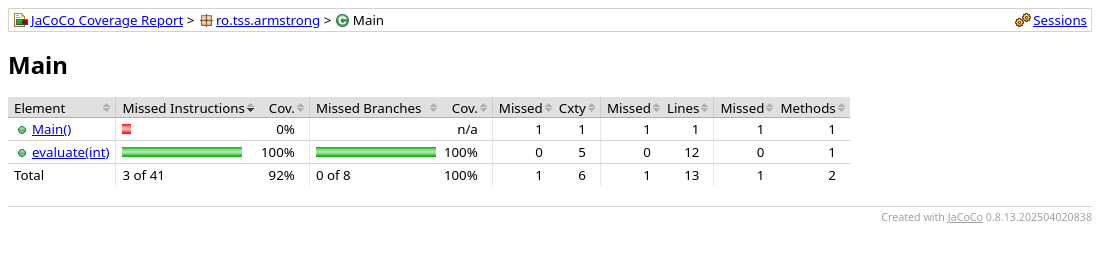
\includegraphics[width=\linewidth]{figuri/coverage_bvatest_v02.png}
\par\small Raport JaCoCo pentru suita Boundary value analysis
\end{center}


\section{Graful cauză--efect}
\textbf{Cauze:}
\begin{itemize}[label=\textendash]
\item $C_1$: $n$ este în intervalul valid, $100\leq n\leq999$
\item $C_2$: $n$ este egal cu suma cuburilor cifrelor sale
\end{itemize}

\textbf{Efecte:}
\begin{itemize}[label=\textendash]
\item $E_1$: mesajul \texttt{INVALID}
\item $E_2$: mesajul \texttt{DA}
\item $E_3$: mesajul \texttt{NU}
\end{itemize}

\textbf{Desenul grafului cauză--efect:}
\begin{center}
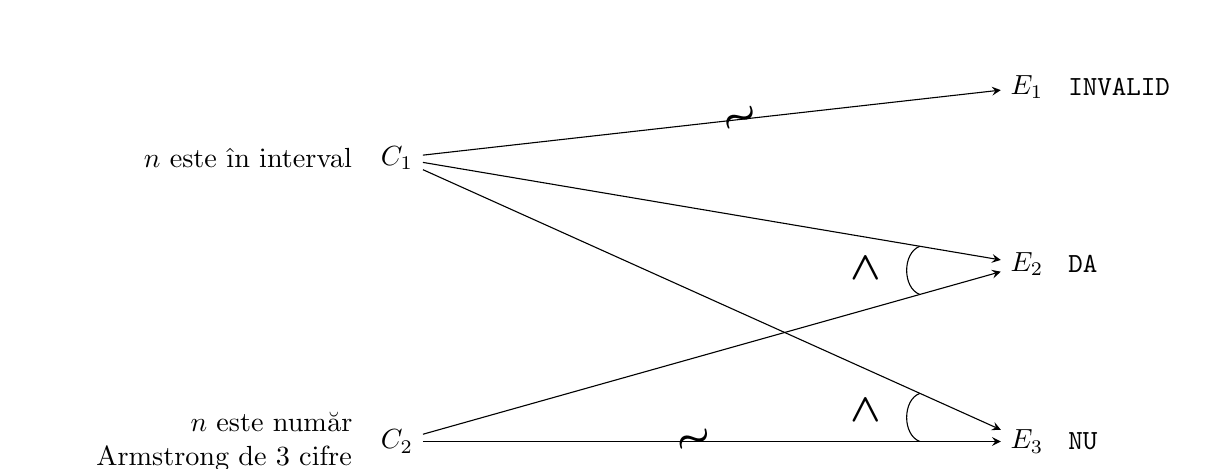
\begin{tikzpicture}[x=1cm,y=1cm,>=stealth,every node/.style={font=\normalsize}]
\node (c1) at (0,0) {$C_1$};
\node (c2) at (0,-3.6) {$C_2$};
\node[anchor=east,align=right,text width=4cm] at (-0.45,0) {$n$ este în interval};
\node[anchor=east,align=right,text width=4cm] at (-0.45,-3.6) {$n$ este număr\\ Armstrong de 3 cifre};
\node (e1) at (8,0.9) {$E_1$};
\node (e2) at (8,-1.35) {$E_2$};
\node (e3) at (8,-3.6) {$E_3$};
\draw[->] (c1) -- node[pos=.55,sloped,rotate=20,fill=none,inner sep=0pt,font=\Large] {$\boldsymbol{\sim}$} (e1);
\draw[->] (c1) -- coordinate[pos=.86] (and2top) (e2);
\draw[->] (c2) -- coordinate[pos=.86] (and2bottom) (e2);
\draw (and2top) to[out=200,in=160] (and2bottom);
\node[font=\Large] at (5.95,-1.4) {$\boldsymbol{\land}$};
\draw[->] (c1) -- coordinate[pos=.86] (and3top) (e3);
\draw[->] (c2) -- node[pos=.47,sloped,rotate=20,fill=none,inner sep=0pt,font=\Large] {$\boldsymbol{\sim}$}
    coordinate[pos=.86] (and3bottom) (e3);
\draw (and3top) to[out=200,in=160] (and3bottom);
\node[font=\Large] at (5.95,-3.2) {$\boldsymbol{\land}$};
\node[anchor=west] at (8.4,0.9) {\texttt{INVALID}};
\node[anchor=west] at (8.4,-1.35) {\texttt{DA}};
\node[anchor=west] at (8.4,-3.6) {\texttt{NU}};
\end{tikzpicture}
\end{center}


\textbf{Construirea tabelelor de decizie:}
\begin{enumerate}[label={\arabic*.},ref=\arabic*,leftmargin=*]
\item $E_1=$ \texttt{INVALID}
  \begin{enumerate}[label={\theenumi.\arabic*.},leftmargin=*,nosep]
  \item $\neg C_1=1 \Rightarrow C_1=0$
  \item Valoarea lui $C_2$ nu contează și se notează cu --
  \end{enumerate}
  \begin{center}
  \begin{tabular}{@{}lc@{}}
  \toprule
  Cauză & Regula 1 \\
  \midrule
  $C_1$ & 0 \\
  $C_2$ & -- \\
  \midrule
  $E_1=\neg C_1$ & 1 \\
  $E_2=C_1\land C_2$ & 0 \\
  $E_3=C_1\land\neg C_2$ & 0 \\
  \bottomrule
  \end{tabular}
  \end{center}

\item $E_2=$ \texttt{DA}
  \begin{enumerate}[label={\theenumi.\arabic*.},leftmargin=*,nosep]
  \item $C_1\land C_2=1 \Rightarrow C_1=1$ și $C_2=1$
  \end{enumerate}
  \begin{center}
  \begin{tabular}{@{}lcc@{}}
  \toprule
  Cauză & Regula 1 & Regula 2 \\
  \midrule
  $C_1$ & 0 & 1 \\
  $C_2$ & -- & 1 \\
  \midrule
  $E_1=\neg C_1$ & 1 & 0 \\
  $E_2=C_1\land C_2$ & 0 & 1 \\
  $E_3=C_1\land\neg C_2$ & 0 & 0 \\
  \bottomrule
  \end{tabular}
  \end{center}

\item $E_3=$ \texttt{NU}
  \begin{enumerate}[label={\theenumi.\arabic*.},leftmargin=*,nosep]
  \item $C_1\land\neg C_2=1 \Rightarrow C_1=1$ și $C_2=0$
  \end{enumerate}
  \begin{center}
  \begin{tabular}{@{}lccc@{}}
  \toprule
  Cauză & Regula 1 & Regula 2 & Regula 3 \\
  \midrule
  $C_1$ & 0 & 1 & 1 \\
  $C_2$ & -- & 1 & 0 \\
  \midrule
  $E_1=\neg C_1$ & 1 & 0 & 0 \\
  $E_2=C_1\land C_2$ & 0 & 1 & 0 \\
  $E_3=C_1\land\neg C_2$ & 0 & 0 & 1 \\
  \bottomrule
  \end{tabular}
  \end{center}

\end{enumerate}

\textbf{Tabel de decizie final și teste:}
\begin{center}
\begin{tabular}{@{}lccc@{}}
\toprule
Cauză & Regula 1 & Regula 2 & Regula 3 \\
\midrule
$C_1$ & 0 & 1 & 1 \\
$C_2$ & -- & 1 & 0 \\
\midrule
$E_1=\neg C_1$ & 1 & 0 & 0 \\
$E_2=C_1\land C_2$ & 0 & 1 & 0 \\
$E_3=C_1\land\neg C_2$ & 0 & 0 & 1 \\
\midrule
Date de intrare $n$ & 99 & 153 & 100 \\
Output & \texttt{INVALID} & \texttt{DA} & \texttt{NU} \\
Test & CEG01 & CEG03 & CEG02 \\
\bottomrule
\end{tabular}
\end{center}

\begin{minipage}{\linewidth}
\textbf{Implementarea testelor și raportul de acoperire}
\begin{lstlisting}[language=Java,firstnumber=1]
public class CauseEffectGraphing {
    @Test
    public void CEG01() {
        assertEquals("INVALID", Main.evaluate(99));
    }

    @Test
    public void CEG02() {
        assertEquals("NU", Main.evaluate(100));
    }

    @Test
    public void CEG03() {
        assertEquals("DA", Main.evaluate(153));
    }

}
\end{lstlisting}

\textbf{Rezultatul execuției:} \texttt{OK (3 tests)}

\begin{center}
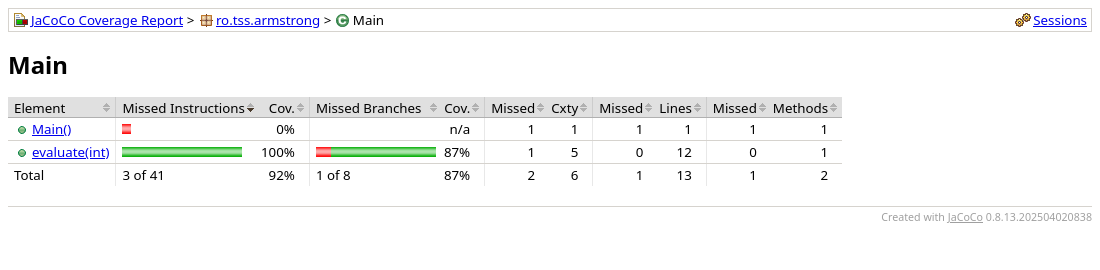
\includegraphics[width=\linewidth]{figuri/coverage_cegtest_v02.png}
\par\small Raport JaCoCo pentru suita Cause-effect graphing
\end{center}
\end{minipage}


\par\vspace{\baselineskip}
\textbf{Interpretarea acoperirii suitei CauseEffectGraphing} \\
Suita verifică toate cele trei efecte ale specificației, utilizând intrările $99$, $100$ și $153$.
Execuția testelor parcurge toate instrucțiunile și liniile metodei,
dar numai șapte dintre cele opt ramuri măsurate de JaCoCo.
Acoperirea ramurilor este, prin urmare, de $87{,}5\%$.

Ramura neacoperită este rezultatul adevărat al condiției \texttt{n > 999}.
Pentru $n=99$, condiția \texttt{n < 100} este adevărată, iar evaluarea
scurtcircuitată a operatorului \texttt{||} împiedică evaluarea celei de-a doua
condiții. Pentru intrările valide $100$ și $153$, condiția \texttt{n > 999}
este evaluată, dar rezultatul său este fals. Astfel, verificarea tuturor
efectelor din tabelul de decizie nu garantează parcurgerea fiecărei ramuri
a implementării. Adăugarea cazului $n=1000$, cu rezultatul așteptat
\texttt{INVALID}, ar determina evaluarea condiției \texttt{n > 999} ca
adevărată și ar crește procentul la $100\%$.



\clearpage
\section{Implementarea programului în cod}

\begin{lstlisting}[language=Java,firstnumber=1]
public static String evaluate(int n) {
    if (n < 100 || n > 999) {
        return "INVALID";
    }
    int rest = n;
    int suma = 0;
    while (rest > 0) {
        int cifra = rest % 10;
        suma += cifra * cifra * cifra;
        rest /= 10;
    }
    if (suma == n) {
        return "DA";
    }
    return "NU";
}
\end{lstlisting}


\subsection{Graful orientat al programului}

\begin{center}
\begin{tikzpicture}[x=1cm,y=0.72cm,>=stealth,
 every node/.style={font=\large,inner sep=3pt},every path/.style={thick}]
\node (n1) at (0,0) {1};
\node (n2) at (0,-1) {2};
\node (n3) at (-3,-2.1) {3};
\node (n4) at (0,-2.1) {4};
\node (n5) at (0,-3.1) {5};
\node (n6) at (0,-4.1) {6};
\node (n7) at (0,-5.1) {7};
\node (n8) at (3,-6.1) {8};
\node (n9) at (3,-7.1) {9};
\node (n10) at (3,-8.1) {10};
\node (n11) at (0,-9.1) {11};
\node (n12) at (0,-10.1) {12};
\node (n13) at (-1.5,-11.95) {13};
\node (n14) at (1.5,-11.3) {14};
\node (n15) at (1.5,-12.3) {15};
\node (n16) at (0,-13.8) {16};
\draw[->] (n1) -- (n2);
\draw[->] (n2) -- node[above left,font=\small] {T} (n3);
\draw[->] (n2) -- node[pos=.55,right=3pt,font=\small] {F} (n4);
\draw[->] (n4) -- (n5);
\draw[->] (n3) |- (n16);
\draw[->] (n5) -- (n6);
\draw[->] (n6) -- (n7);
\draw[->] (n7) -- node[below left,font=\small] {T} (n8);
\draw[->] (n7) -- node[left,font=\small] {F} (n11);
\draw[->] (n8) -- (n9);
\draw[->] (n9) -- (n10);
\draw[->] (n11) -- (n12);
\draw[->] (n10) -- (4.2,-8.1) -- (4.2,-5.1) -- (n7);
\draw[->] (n12) -- node[above left,font=\small] {T} (n13);
\draw[->] (n12) -- node[above right,font=\small] {F} (n14);
\draw[->] (n14) -- (n15);
\draw[->] (n13) -- (n16);
\draw[->] (n15) -- (n16);
\end{tikzpicture}

\end{center}

\clearpage
\section{Deciziile programului}
Pentru fiecare decizie, tabelul prezintă valorile condițiilor individuale,
rezultatul deciziei și datele care realizează combinația respectivă.
Liniile corespund
codului din capitolul 5 și nodurilor grafului.

\textbf{Decizia D1, linia 2:}
\[
\begin{gathered}
D_1=\{n\in\mathbb{N}\mid n<100\lor n>999\}=C_1\lor C_2
\\[2pt]
\text{unde}\quad C_1=\{n\in\mathbb{N}\mid n<100\}\text{ și }C_2=\{n\in\mathbb{N}\mid n>999\}
\end{gathered}
\]

\begin{center}
\begin{tabular}{@{}lllll@{}}
\toprule
Caz & $C_1$ & $C_2$ & $D_1$ & Date intrare \\
\midrule
T1 & true & true & true & Combinație imposibilă \\
T2 & false & false & false & $n=100$ \\
T3 & false & true & true & $n=1000$ \\
T4 & true & false & true & $n=99$ \\
\bottomrule
\end{tabular}
\end{center}

\textbf{Decizia D2, linia 7:}
\[
\begin{gathered}
D_2=\{\texttt{rest}\in\mathbb{N}\mid\texttt{rest}>0\}=C_3
\\[2pt]
\text{unde}\quad C_3=\{\texttt{rest}\in\mathbb{N}\mid\texttt{rest}>0\}
\end{gathered}
\]

\begin{center}
\begin{tabular}{@{}llll@{}}
\toprule
Caz & $C_3$ & $D_2$ & Date intrare \\
\midrule
T5 & true & true & $n=100$, $\texttt{rest}=100$, înaintea primei iterații \\
T6 & false & false & $n=100$, $\texttt{rest}=0$, după a treia iterație \\
\bottomrule
\end{tabular}
\end{center}


\textbf{Decizia D3, linia 12:}
\[
\begin{gathered}
D_3=\{n\in\mathbb{N},\ \texttt{suma}\in\mathbb{N}\mid\texttt{suma}=n\}=C_4
\\[2pt]
\text{unde}\quad C_4=\{n\in\mathbb{N},\ \texttt{suma}\in\mathbb{N}\mid\texttt{suma}=n\}
\end{gathered}
\]

\begin{center}
\begin{tabular}{@{}llll@{}}
\toprule
Caz & $C_4$ & $D_3$ & Date intrare \\
\midrule
T7 & true & true & $n=153$, $\texttt{suma}=153$ \\
T8 & false & false & $n=100$, $\texttt{suma}=1$ \\
\bottomrule
\end{tabular}
\end{center}

\textbf{Setul de teste rezultat:} $n\in\{99,100,1000,153\}$

\subsection{Implementarea testelor și acoperirea măsurată}
Cele patru teste JUnit de mai jos verifică rezultatele așteptate pentru
intrările din analiza deciziilor. 
\begin{itemize}[label=\textbullet]
\item Cazul $n=100$ acoperă \textbf{T2}, \textbf{T5}, \textbf{T6} și \textbf{T8}
\item Cazul $n=153$ acoperă \textbf{T7}
\item Cazul $n=99$ acoperă \textbf{T4}
\item Cazul $n=1000$ acoperă \textbf{T3}
\item \textbf{T1} este o combinație imposibilă și nu poate fi realizat de o intrare
\end{itemize}

\clearpage
\begin{lstlisting}[language=Java,firstnumber=1]
public class ModifiedConditionDecisionCoverage {
    @Test public void cazul_001() {
        assertEquals("NU", Main.evaluate(100));
    }
    @Test public void cazul_002() {
        assertEquals("DA", Main.evaluate(153));
    }
    @Test public void cazul_003() {
        assertEquals("INVALID", Main.evaluate(99));
    }
    @Test public void cazul_004() {
        assertEquals("INVALID", Main.evaluate(1000));
    }
}
\end{lstlisting}

\textbf{Rezultatul execuției:} \texttt{OK (4 tests)}

\begin{center}
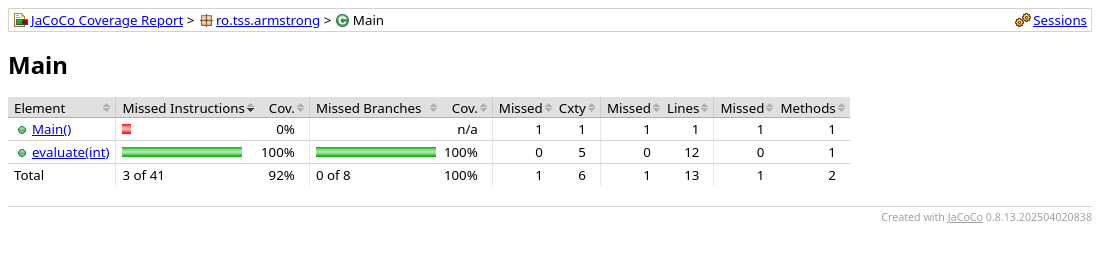
\includegraphics[width=\linewidth]{figuri/coverage_mcdc_armstrong_v03.png}
\par\small Captură din raportul JaCoCo al suitei \texttt{Modified\allowbreak{}Condition\allowbreak{}Decision\allowbreak{}Coverage}
\end{center}


\subsection{Complexitatea ciclomatică}
Graful orientat al programului conține $N=16$ noduri și $E=18$ arce.
Nodurile sunt numerotate după liniile metodei din capitolul 5:
\[
\{1,2,3,4,5,6,7,8,9,10,11,12,13,14,15,16\}
\]
Nodul 1 reprezintă intrarea în metodă, iar nodul 16 este ieșirea comună
celor trei instrucțiuni de returnare. Nodurile 4 și 14 reprezintă închiderile blocurilor condiționale, pe
ramurile false: $2\to4\to5$, respectiv $12\to14\to15$.
Graful are o singură componentă conexă.

Calculăm complexitatea ciclomatică prin cele două metode:
\begin{itemize}[label=\textbullet]
\item $V(G)=E-N+2=18-16+2=4$
\item $V(G)=\text{numărul deciziilor binare}+1=3+1=4$
\end{itemize}
Cele trei decizii sunt validarea de la linia 2, condiția buclei de la linia 7
și comparația dintre sumă și numărul inițial de la linia 12.
Condiția compusă de la linia 2 este reprezentată printr-un singur nod,
conform convenției utilizate în graful pe linii.

\subsection{Circuite liniar independente}
Pentru obținerea grafului derivat, adăugăm arcul fictiv $16\to1$, care
conectează ieșirea cu intrarea. Graful rezultat este tare conex:
din orice nod se poate ajunge la ieșire și, prin arcul adăugat,
la intrare și la celelalte noduri. Arcul fictiv este folosit numai
în analiza circuitelor și nu reprezintă o instrucțiune executabilă.

Graful derivat are $E'=19$ arce, iar dimensiunea spațiului circuitelor este
\[
E'-N+1=19-16+1=4=V(G)
\]
O bază de patru circuite liniar independente este:
\begin{itemize}[label=\textbullet]
\item $c_1:\ 1\to2\to3\to16\to1$
\item $c_2:\ 1\to2\to4\to5\to6\to7\to11\to12\to13\to16\to1$
\item $c_3:\ 1\to2\to4\to5\to6\to7\to11\to12\to14\to15\to16\to1$
\item $c_4:\ 7\to8\to9\to10\to7$
\end{itemize}
Fiecare circuit conține un arc care nu apare în celelalte:
\begin{itemize}[label=\textbullet]
\item pentru $c_1$: $2\to3$
\item pentru $c_2$: $12\to13$
\item pentru $c_3$: $12\to14$
\item pentru $c_4$: $7\to8$
\end{itemize}
Prin urmare, vectorii lor de incidență sunt
liniar independenți. Reuniunea celor patru circuite conține toate cele
19 arce ale grafului derivat.

\textbf{Legătura cu testele existente}
\begin{center}
\begin{tabular}{@{}llll@{}}
\toprule
Test & $n$ & Rezultat & Descompunerea traseului în circuite \\
\midrule
EP03 & 99 & \texttt{INVALID} & $c_1$ \\
EP01 & 153 & \texttt{DA} & $c_2$ și 3 parcurgeri ale lui $c_4$ \\
BVA02 & 100 & \texttt{NU} & $c_3$ și 3 parcurgeri ale lui $c_4$ \\
\bottomrule
\end{tabular}
\end{center}
Tabelul descrie traseele închise prin arcul fictiv $16\to1$.
Pentru $n=153$, variabila \texttt{rest} ia succesiv valorile $153,15,1,0$;
pentru $n=100$, valorile sunt $100,10,1,0$.
Astfel, circuitul $c_4$ este parcurs de trei ori înainte de ieșirea din buclă.
Circuitele $c_2$ și $c_3$ descriu partea traseului rămasă după eliminarea
acestor parcurgeri ale buclei. Ele nu sunt executabile separat cu zero
iterații pentru o intrare validă de trei cifre.


\section{Mutanți echivalenți și ne-echivalenți}
Fiecare mutant de mai jos este de ordinul 1: se modifică un singur operator
al programului original. Numerele liniilor se referă la metoda prezentată
în capitolul 5.

Pentru cei doi mutanți ne-echivalenți folosim același test,
\texttt{BVA02}, cu intrarea $n=100$ și rezultatul așteptat \texttt{NU}:
\begin{lstlisting}[language=Java,firstnumber=1]
@Test
public void BVA02() {
    assertEquals("NU", Main.evaluate(100));
}
\end{lstlisting}
Pe programul original, suma cuburilor cifrelor lui 100 este 1,
iar $1\ne100$, deci testul trece.

\subsection{Mutant echivalent}
Modificăm operatorul \texttt{||} de la linia 2 în \texttt{|}.

\textbf{Instrucțiunea originală}
\begin{lstlisting}[language=Java,firstnumber=2]
if (n < 100 || n > 999) {
\end{lstlisting}
\textbf{Instrucțiunea modificată}
\begin{lstlisting}[language=Java,firstnumber=2]
if ((n < 100 | n > 999)) {
\end{lstlisting}
Pentru operanzi booleeni, cei doi operatori au aceeași tabelă de adevăr.
Diferența este că \texttt{||} scurtcircuitează evaluarea, în timp ce
\texttt{|} evaluează ambele comparații. Comparațiile sunt definite pentru
orice valoare de tip \texttt{int}, nu modifică starea programului și nu
produc excepții. Prin urmare, rezultatul metodei este identic cu cel al
originalului pentru orice intrare. 

\subsection{Mutant ne-echivalent, omorât de test}
Modificăm operatorul \texttt{<} de la linia 2 în \texttt{<=}:
\begin{lstlisting}[language=Java,firstnumber=2]
if (n <= 100 || n > 999) {
\end{lstlisting}
Pentru $n=100$, validarea mutantului respinge intrarea și întoarce
\texttt{INVALID}, în timp ce originalul întoarce \texttt{NU}.
Aserțiunea din \texttt{BVA02} eșuează, deci testul omoară mutantul.
Aceeași intrare constituie un martor al neechivalenței.

\subsection{Mutant ne-echivalent, neomorât de același test}
Modificăm operatorul \texttt{>} de la linia 2 în \texttt{>=}:
\begin{lstlisting}[language=Java,firstnumber=2]
if (n < 100 || n >= 999) {
\end{lstlisting}
Pentru $n=100$, atât originalul, cât și mutantul întorc \texttt{NU},
așadar \texttt{BVA02} nu detectează modificarea.
Totuși, mutantul nu este echivalent: pentru $n=999$, originalul calculează
$9^3+9^3+9^3=2187\ne999$ și întoarce \texttt{NU}, iar mutantul întoarce
\texttt{INVALID}. Testul \texttt{BVA15}, cu această intrare, îl omoară.

\subsection{Rezultatele verificării}
\begin{center}
\begin{tabular}{@{}lccl@{}}
\toprule
Variantă & \shortstack{BVA02\\[3pt]$n=100$} & \shortstack{BVA15\\[3pt]$n=999$} & Clasificare \\
\midrule
Original & \texttt{NU} & \texttt{NU} & Referință \\
Mutant echivalent & \texttt{NU} & \texttt{NU} & Echivalent \\
Mutant omorât & \texttt{INVALID} & \texttt{NU} & Neechivalent \\
Mutant supraviețuitor & \texttt{NU} & \texttt{INVALID} & Neechivalent \\
\bottomrule
\end{tabular}
\end{center}


\clearpage
\section{Mutation Tools}
\label{sec:mutation-tools}
Testarea de mutație evaluează capacitatea testelor de a detecta modificări
ale programului. Un operator de mutație introduce o modificare locală,
precum schimbarea unei comparații sau a unei operații aritmetice.
Testele sunt apoi executate asupra variantei modificate. Dacă rezultatul
observat nu mai respectă aserțiunile, mutantul este detectat.

Pentru metoda \texttt{Main.evaluate(int n)} au fost utilizate două unelte
distincte: \textbf{PIT 1.17.4} și \textbf{Major 3.0.1}.
Analiza urmărește cele trei suite funcționale, EP, BVA și CEG,
precum și suita MC/DC. 

\subsection{Obiectivul și protocolul experimental}
Programul original întoarce \texttt{DA}, \texttt{NU} sau \texttt{INVALID}.
Testele compară valoarea returnată cu un rezultat așteptat explicit.
Prin urmare, simpla executare a unei linii nu este suficientă pentru
detectarea unui mutant: modificarea trebuie să influențeze un rezultat
verificat sau terminarea execuției.

\textbf{Suitele analizate}
\begin{center}
\begingroup\small
\begin{tabular}{@{}llr@{}}
\toprule
Metodă & Clasă JUnit & Teste \\
\midrule
EP & \texttt{EquivalncePartitioning} & 4 \\
BVA & \texttt{BoundaryValueAnalysis} & 16 \\
CEG & \texttt{CauseEffectGraphing} & 3 \\
MC/DC & \texttt{ModifiedConditionDecisionCoverage} & 4 \\
\bottomrule
\end{tabular}
\endgroup
\end{center}
Toate clasele aparțin pachetului \path{ro.tss.armstrong}.
Cele patru suite conțin în total 27 de metode JUnit, unele cu intrări comune.
Separat, \texttt{RegressionTest} verifică 902 intrări: toate cele 900 de valori
valide și vecinii exteriori 99 și 1000. Regresia este folosită ca verificare
suplimentară a originalului, fără a fi cumulată cu suitele din comparația
scorurilor de mutație. Cu această metodă suplimentară, rularea JUnit are
28 de teste trecute.

Protocolul este următorul:
\begin{enumerate}[label=\arabic*.,leftmargin=*]
\item Se compilează originalul și testele și se verifică trecerea tuturor aserțiunilor
\item PIT generează mutanți pentru clasa \path{ro.tss.armstrong.Main}, cu constructorul exclus
\item Major compilează aceeași sursă folosind configurația \path{all.mml.bin}
\item Fiecare unealtă analizează separat EP, BVA, CEG și MC/DC
\item Se păstrează rapoartele brute, operatorul, localizarea și statutul fiecărui mutant
\item Se recalculează scorurile cu aceeași convenție pentru ambele unelte și se verifică martori ai neechivalenței
\end{enumerate}

PIT produce 15 mutanți, iar Major 31. 
În total avem 8 analize, cu $4\times15+4\times31=184$ înregistrări de rezultate.
Numărul 184 include analiza repetată a aceluiași mutant cu suite diferite,
nu 184 de modificări distincte ale programului.

\subsection{Semnificația statuturilor și calcularea scorurilor}
Pentru fiecare analiză folosim următoarele notații:
\begin{itemize}[label=\textbullet]
\item $G$: numărul total de mutanți generați și analizați
\item $K$: mutanții omorâți prin eșecul unei aserțiuni sau printr-o excepție
\item $T$: mutanții pentru care execuția depășește limita de timp
\item $S$: mutanții supraviețuitori, pentru care testele executate trec
\item $U$: mutanții fără acoperire, al căror cod nu este atins de suită
\item $E$: mutanții echivalenți demonstrați, incluși inițial între supraviețuitori
\end{itemize}
În toate rulările de față se verifică identitatea
\[
G=K+T+S+U
\]
Un supraviețuitor nu este automat echivalent. El poate reprezenta fie o
modificare fără efect observabil pentru orice intrare, fie un defect pe care
intrările suitei nu îl evidențiază. Statutul de timeout necesită, de asemenea,
interpretare: poate indica o buclă infinită introdusă de mutant sau o limită
de timp insuficientă. În acest experiment, modificările care produc timeout
sunt identificate și explicate pe cod.

\subsubsection{Scorul brut, cu timeout-uri considerate detectări}
Scorul de mutație, notat $MS$ (\emph{mutation score}), reprezintă procentul mutanților detectați de o suită de teste din totalul mutanților generați și analizați. În acord cu totalurile afișate de uneltele utilizate, considerăm detectați atât mutanții omorâți prin eșecul unei aserțiuni sau printr-o excepție ($K$), cât și cei pentru care execuția depășește limita de timp ($T$):
\[
MS=\frac{K+T}{G}\times100\%
\]
Dacă originalul termină pentru o intrare, iar mutantul introduce o buclă
infinită, schimbarea este observabilă, chiar dacă nu se ajunge la o aserțiune.
De aceea, coloanele $K$ și $T$ rămân distincte în tabele, iar calculul
scorului folosește explicit suma lor. \href{https://pitest.org/quickstart/basic_concepts/}{PIT}
prezintă separat stările \texttt{Killed}, \texttt{Survived},
\texttt{No coverage} și \texttt{Timed Out}, în timp ce Major raportează
agregatul \texttt{FAIL--EXC--TIME} pentru mutanții detectați.

Indicatorul $TS$ (\emph{test strength}) raportează detectările numai la mutanții
atinși de teste:
\[
TS=\frac{K+T}{G-U}\times100\%
\]
În toate cele opt rulări, $U=0$. În consecință, $TS$ și $MS$ au aceeași
valoare numerică în acest experiment. Această egalitate nu implică faptul
că cele două măsuri sunt întotdeauna identice.

\subsubsection{Convenția fără timeout din rapoartele existente}
În continuare, termenul \emph{scor brut} desemnează \emph{scorul de mutație} ($MS$).
Scorurile fără timeout sunt etichetate separat, pentru a evita compararea
unor procente calculate cu numitori diferiți.
\[
MS_{\text{fără timeout}}=\frac{K}{G-T}\times100\%
\]
Aceasta elimină timeout-urile atât din numărător, cât și din numitor.
Diferența față de scorul brut de mai sus provine din formulă, nu dintr-o
nouă selecție de teste.

\begin{center}
\begingroup\small
\begin{tabular}{@{}llcc@{}}
\toprule
Unealtă & Suită & $K/(G-T)$ & Scor fără timeout \\
\midrule
PIT & EP & 12/14 & 85,7\% \\
Major & EP & 25/29 & 86,2\% \\
PIT & BVA & 14/14 & 100,0\% \\
Major & BVA & 28/29 & 96,6\% \\
PIT & CEG & 13/14 & 92,9\% \\
Major & CEG & 24/29 & 82,8\% \\
PIT & MC/DC & 13/14 & 92,9\% \\
Major & MC/DC & 26/29 & 89,7\% \\
\bottomrule
\end{tabular}
\endgroup
\end{center}


\subsection{PIT: configurare și utilizare}
\subsubsection{Mediul și selecția codului analizat}
PIT este utilizat prin interfața de linie de comandă, cu biblioteca
\path{pitest-command-line-1.17.4.jar} și dependențele locale aferente.
Scriptul \path{main/tools/run.py} lansează clasa
\path{org.pitest.mutationtest.commandline.MutationCoverageReport}.
Originalul și testele sunt compilate cu JDK 17 și opțiunea \texttt{--release 11},
care produce clase compatibile cu Java 11. 

Selecția este limitată la \path{ro.tss.armstrong.Main}.
În această clasă, metoda analizată este \texttt{evaluate}; constructorul
implicit este exclus prin \texttt{--excludedMethods <init>}.
Clasa JUnit este selectată explicit pentru fiecare rulare.
De exemplu, pentru BVA, opțiunile relevante sunt:
\begin{lstlisting}[language=,numbers=none]
--targetClasses ro.tss.armstrong.Main
--targetTests ro.tss.armstrong.BoundaryValueAnalysis
--mutableCodePaths .../target/classes
--sourceDirs .../src/main/java
--excludedMethods <init>
--outputFormats XML,HTML
--timestampedReports false
--threads 2
--timeoutConst 1000
\end{lstlisting}

\subsubsection{Operatorii care au produs efectiv mutanți}
PIT modifică bytecode-ul rezultat din compilare, apoi execută testele
asupra clasei modificate. Cele 15 mutații observate aparțin următoarelor
patru familii:
\begin{itemize}[label=\textbullet]
\item \textbf{Conditionals Boundary}: modificarea limitelor comparațiilor, de exemplu \texttt{n < 100} în \texttt{n <= 100}
\item \textbf{Negate Conditionals}: inversarea rezultatului unei condiții
\item \textbf{Math}: înlocuirea unor operații aritmetice, inclusiv în actualizările variabilelor
\item \textbf{Empty Object Return Values}: înlocuirea rezultatului de tip \texttt{String} cu șirul vid
\end{itemize}
Configurația implicită poate conține și alți operatori, dar aceștia nu au
produs mutanți suplimentari pentru metoda de față.

Tabelul următor arată numărul de mutanți generați de fiecare operator și
numărul de detectări $K+T$ pentru fiecare suită:
\begin{center}
\begingroup\small
\begin{tabular}{@{}lccccc@{}}
\toprule
Operator & $G$ & EP & BVA & CEG & MC/DC \\
\midrule
Conditionals\allowbreak{}Boundary & 3 & 1/3 & 3/3 & 2/3 & 2/3 \\
Empty\allowbreak{}ObjectReturnVals & 3 & 3/3 & 3/3 & 3/3 & 3/3 \\
Math & 5 & 5/5 & 5/5 & 5/5 & 5/5 \\
Negate\allowbreak{}Conditionals & 4 & 4/4 & 4/4 & 4/4 & 4/4 \\
\bottomrule
\end{tabular}
\endgroup
\end{center}

Cei 3 mutanți Boundary sunt cei ai limitelor inferioară și superioară
ale intrării și cel al condiției buclei.
Cele 5 mutații Math privesc extragerea cifrei prin \texttt{\%}, cele două înmulțiri din cub, adunarea în \texttt{suma} și împărțirea care actualizează \texttt{rest}.
Cele trei mutații ale valorii returnate corespund rezultatelor
\texttt{INVALID}, \texttt{DA} și \texttt{NU}.

\subsubsection{Rezultatele celor patru suite}
\begin{center}
\begingroup\small
\begin{tabular}{@{}lcccccc@{}}
\toprule
Suită & $G$ & $K$ & $T$ & $S$ & $U$ & $MS$ \\
\midrule
EP & 15 & 12 & 1 & 2 & 0 & 13/15 = 86,7\% \\
BVA & 15 & 14 & 1 & 0 & 0 & 15/15 = 100,0\% \\
CEG & 15 & 13 & 1 & 1 & 0 & 14/15 = 93,3\% \\
MC/DC & 15 & 13 & 1 & 1 & 0 & 14/15 = 93,3\% \\
\bottomrule
\end{tabular}
\endgroup
\end{center}

Pentru EP, cele 12 detectări prin aserțiuni se completează cu un timeout,
rezultând $MS=(12+1)/15=86{,}7\%$.
Pentru BVA, niciun mutant nu supraviețuiește: 14 sunt omorâți direct,
iar unul produce timeout, deci $MS=15/15=100\%$.
CEG și MC/DC au fiecare 13 mutanți omorâți direct, un timeout și un
supraviețuitor, adică $MS=14/15=93{,}3\%$.

Absența mutanților fără acoperire nu contrazice procentul de $87{,}5\%$
al ramurilor pentru CEG. Starea \texttt{No coverage} privește atingerea
codului în care se află mutația, nu realizarea fiecărui rezultat logic.
CEG ajunge la validare, dar nu furnizează o valoare peste 999;
mutantul limitei superioare este astfel supraviețuitor, nu neacoperit.

Rezultatul arată că suita cu 100\% acoperire a ramurilor poate lăsa totuși
mutanți în viață. EP și MC/DC au această acoperire structurală,
dar nu conțin toate valorile care disting comparațiile originale de
versiunile cu limite modificate.

\subsubsection{Supraviețuitori și teste care evidențiază diferențele}
\textbf{Modificarea limitei inferioare}
\begin{lstlisting}[language=Java,firstnumber=2]
if (n <= 100 || n > 999) {
\end{lstlisting}
Acest mutant supraviețuiește suitei EP. Intrările EP sunt $153$, $123$,
$99$ și $1000$, iar pentru ele rezultatele originalului și mutantului coincid.
Valoarea $100$ lipsește. Testul \texttt{BVA02}, cu $n=100$,
așteaptă \texttt{NU}, în timp ce mutantul întoarce \texttt{INVALID}.
Aceeași intrare este prezentă în CEG și MC/DC, motiv pentru care mutantul
este detectat și de aceste suite.

\textbf{Modificarea limitei superioare}
\begin{lstlisting}[language=Java,firstnumber=2]
if (n < 100 || n >= 999) {
\end{lstlisting}
Acest mutant supraviețuiește în EP, CEG și MC/DC.
Niciuna dintre cele trei suite nu conține $n=999$.
\texttt{BVA15} verifică această valoare: originalul întoarce \texttt{NU},
întrucât suma cuburilor este 2187, iar mutantul întoarce \texttt{INVALID}.
Prin urmare, supraviețuirea indică o lipsă concretă a selecției de teste,
nu echivalența mutantului.

\textbf{Timeout-ul condiției buclei}
PIT schimbă \texttt{rest > 0} în \texttt{rest >= 0}.
După procesarea celor trei cifre, \texttt{rest} devine 0.
Noua condiție rămâne adevărată, iar instrucțiunea \texttt{rest /= 10}
păstrează valoarea 0. Execuția nu se mai termină.
Fiecare suită conține cel puțin o intrare validă și detectează acest mutant
prin timeout. Explicația se bazează pe actualizarea variabilei din cod,
nu doar pe eticheta raportului.

Toți cei 15 mutanți sunt detectați de BVA, fie prin rezultat, fie prin
neterminare. 

\subsection{Major: configurare și utilizare}
\subsubsection{Generarea mutanților la compilare}
Major este utilizat în versiunea 3.0.1, cu un JDK 11 local proiectului.
Sursa analizată este aceeași clasă \texttt{Main}, iar testele sunt cele
executate și cu PIT. Nu se modifică aserțiunile și nu se înlocuiesc datele
pentru a favoriza una dintre unelte.

Major introduce mutațiile în timpul compilării sursei și le include în
clasele instrumentate. Configurația este exprimată prin MML, limbajul
specific al uneltei. 
În proiect, comanda apelată de script are forma:
\begin{lstlisting}[language=,numbers=none]
.tools/major/bin/major \
  --mml .tools/major/mml/all.mml.bin \
  --release 11 -g \
  -d 14_armstrong/target/major-classes \
  14_armstrong/src/main/java/ro/tss/armstrong/Main.java
\end{lstlisting}

Fișierul \path{all.mml.bin} este configurația compilată livrată cu
Major. Sursa sa, \path{all.mml}, activează familiile AOR, LOR, SOR,
COR, ROR, LVR, ORU și STD și stabilește înlocuirile permise.
În programul Armstrong, raportul efectiv conține mutanți numai din
AOR, ROR, COR și STD. 

\subsubsection{Operatorii observați și semnificația lor}
\begin{itemize}[label=\textbullet]
\item \textbf{AOR}: înlocuirea operatorilor aritmetici
\item \textbf{ROR}: înlocuirea operatorilor relaționali sau a unor condiții cu valori constante
\item \textbf{COR}: înlocuirea expresiilor condiționale, inclusiv păstrarea unui singur operand
\item \textbf{STD}: eliminarea unor instrucțiuni, precum o atribuire sau un \texttt{return}
\end{itemize}

În total avem 31 de mutanți: 12 AOR, 12 ROR, 3 COR și 4 STD.

Pentru aritmetică, configurația permite mai multe alternative.
De exemplu, expresia \texttt{rest \% 10} generează în această rulare
înlocuiri cu \texttt{*}, \texttt{+}, \texttt{-} și \texttt{/}.
Pentru comparația \texttt{n < 100}, raportul include
\texttt{n != 100}, \texttt{n <= 100} și \texttt{false}.
COR produce, între altele, înlocuirea întregii validări cu un singur operand,
iar STD elimină instrucțiunea \texttt{rest /= 10}.
Aceste modificări nu au toate un corespondent în inventarul implicit PIT
observat pentru aceeași metodă.

În tabelul următor, fiecare celulă a suitei indică detectările $K+T$
raportate la numărul de mutanți ai familiei:
\begin{center}
\begingroup\small
\begin{tabular}{@{}lccccc@{}}
\toprule
Operator & $G$ & EP & BVA & CEG & MC/DC \\
\midrule
AOR & 12 & 12/12 & 12/12 & 12/12 & 12/12 \\
COR & 3 & 3/3 & 3/3 & 2/3 & 3/3 \\
ROR & 12 & 8/12 & 11/12 & 8/12 & 9/12 \\
STD & 4 & 4/4 & 4/4 & 4/4 & 4/4 \\
\bottomrule
\end{tabular}
\endgroup
\end{center}


\subsubsection{Rezultate și motivele detectării}
\begin{center}
\begingroup\small
\begin{tabular}{@{}lcccccc@{}}
\toprule
Suită & $G$ & $K$ & $T$ & $S$ & $U$ & $MS$ \\
\midrule
EP & 31 & 25 & 2 & 4 & 0 & 27/31 = 87,1\% \\
BVA & 31 & 28 & 2 & 1 & 0 & 30/31 = 96,8\% \\
CEG & 31 & 24 & 2 & 5 & 0 & 26/31 = 83,9\% \\
MC/DC & 31 & 26 & 2 & 3 & 0 & 28/31 = 90,3\% \\
\bottomrule
\end{tabular}
\endgroup
\end{center}


Major distinge eșecul unei aserțiuni, excepția și timeout-ul.
Distribuția acestor motive este păstrată separat:
\begin{center}
\begingroup\small
\begin{tabular}{@{}lccccc@{}}
\toprule
Suită & FAIL & EXC & TIME & LIVE & UNCOV \\
\midrule
EP & 25 & 0 & 2 & 4 & 0 \\
BVA & 24 & 4 & 2 & 1 & 0 \\
CEG & 20 & 4 & 2 & 5 & 0 \\
MC/DC & 22 & 4 & 2 & 3 & 0 \\
\bottomrule
\end{tabular}
\endgroup
\end{center}

\texttt{FAIL} și \texttt{EXC} formează împreună $K$.
\texttt{TIME} formează $T$, \texttt{LIVE} formează $S$, iar
\texttt{UNCOV} formează $U$.
Astfel, pentru BVA, cei 30 de mutanți detectați sunt
$24\ \mathrm{FAIL}+4\ \mathrm{EXC}+2\ \mathrm{TIME}$.

Excepțiile sunt relevante pentru corectitudinea programului mutant.
De exemplu, înlocuirea unei înmulțiri cu o împărțire sau un rest poate
introduce împărțirea la zero când cifra procesată este 0.
Originalul este definit pentru toate intrările valide, deci o asemenea
excepție reprezintă un comportament diferit, nu un defect al infrastructurii.
EP conține valorile valide 153 și 123, fără cifra 0, pe când celelalte
suite includ 100. Distribuția \texttt{FAIL}/\texttt{EXC} diferă astfel
chiar atunci când mutantul este detectat de toate suitele.

\subsubsection{Analiza completă a mutanților supraviețuitori}
Reuniunea supraviețuitorilor celor patru suite conține identificatorii
2, 5, 6, 7, 11 și 29. Aceștia sunt analizați individual:

\begin{center}
\begingroup\small
\begin{tabular}{@{}clll@{}}
\toprule
ID & Modificare & Supraviețuiește în & Martor / verdict \\
\midrule
2 & $n<100\to n\leq100$ & EP & $n=100$ \\
5 & $n>999\to n\geq999$ & EP, CEG, MC/DC & $n=999$ \\
6 & $n>999\to\mathrm{false}$ & CEG & $n=1000$ \\
7 & $C_1\lor C_2\to C_1$ & CEG & $n=1000$ \\
11 & $\texttt{rest}>0\to\texttt{rest}\ne0$ & Toate & Echivalent \\
29 & $\texttt{suma}=n\to\texttt{suma}\geq n$ & EP, CEG, MC/DC & $n=154$ \\
\bottomrule
\end{tabular}
\endgroup
\end{center}
Pe rândul 7, $C_1$ și $C_2$ sunt condițiile validării:
$n<100$, respectiv $n>999$.

\textbf{Mutantul 2: limita inferioară}
- Pentru $n=100$, originalul întoarce \texttt{NU}, iar mutantul
\texttt{INVALID}. EP nu conține această limită, deci mutantul supraviețuiește.
\texttt{BVA02}, \texttt{CEG02} și testul MC/DC cu aceeași intrare
îl detectează. Acesta este același tip de defect de frontieră identificat
și de operatorul Boundary din PIT.

\textbf{Mutantul 5: limita superioară}
- Pentru $n=999$, originalul întoarce \texttt{NU}, iar mutantul
\texttt{INVALID}. Numai BVA include această valoare, prin \texttt{BVA15}.
Absența lui 999 explică supraviețuirea în celelalte trei suite.

\textbf{Mutanții 6 și 7: eliminarea validării superioare}
- Înlocuirea lui \texttt{n > 999} cu \texttt{false} și reducerea expresiei
OR la operandul \texttt{n < 100} au același efect observabil aici:
valorile peste 999 nu mai sunt respinse.
Pentru $n=1000$, originalul întoarce \texttt{INVALID}, iar ambii mutanți
calculează suma cuburilor și întorc \texttt{NU}.
Intrarea apare în EP, BVA și MC/DC, dar lipsește din CEG.
Astfel, CEG nu detectează niciunul dintre cei doi mutanți.

\textbf{Mutantul 29: comparația finală}
- Schimbarea \texttt{suma == n} în \texttt{suma >= n} nu este observată
de testele valide din EP, CEG și MC/DC: acestea folosesc fie un număr
Armstrong, fie un număr pentru care suma cuburilor este mai mică decât $n$.
Pentru $n=154$, suma este $1+125+64=190>154$.
Originalul întoarce \texttt{NU}, iar mutantul întoarce \texttt{DA}.
\texttt{BVA06} verifică acest caz și omoară mutantul.

\subsubsection{Demonstrarea echivalenței mutantului 11}
Originalul folosește condiția \texttt{rest > 0}, iar mutantul
\texttt{rest != 0}. După validare, $100\leq n\leq999$ și
\texttt{rest} este inițial egal cu $n$.
La fiecare iterație, împărțirea întreagă la 10 păstrează
$\texttt{rest}\geq0$ și conduce în final la 0.
Pe acest invariant, relațiile
\[
\texttt{rest}>0\quad\text{și}\quad\texttt{rest}\ne0
\]
sunt echivalente. Pentru intrările invalide, metoda întoarce
\texttt{INVALID} înainte de buclă, în ambele variante.
Prin urmare, mutantul 11 păstrează rezultatul și terminarea pentru
orice intrare de tip \texttt{int}.

\subsubsection{Timeout-urile Major}
Toate suitele detectează prin timeout aceiași doi mutanți:
\begin{itemize}[label=\textbullet]
\item ID 12: condiția \texttt{rest > 0} devine \texttt{rest >= 0}, iar bucla continuă după ce variabila ajunge la 0
\item ID 27: este eliminată instrucțiunea \texttt{rest /= 10}, astfel încât variabila rămâne pozitivă și bucla nu mai avansează spre terminare
\end{itemize}

\subsection{Comparația finală PIT versus Major}
\subsubsection{Scoruri brute și scoruri ajustate}
După demonstrarea echivalenței, se poate calcula și scorul ajustat:
\[
MS_{\mathrm{ajustat}}=\frac{K+T}{G-E}\times100\%
\]
În inventarul PIT, $E=0$, astfel încât scorul ajustat coincide cu cel brut.
În inventarul Major, $E=1$ pentru toate suitele, iar numitorul ajustat
este $31-1=30$.
\begin{center}
\begingroup\small
\begin{tabular}{@{}lccc@{}}
\toprule
Suită & PIT brut & Major brut & Major ajustat ($E=1$) \\
\midrule
EP & 86,7\% & 87,1\% & 27/30 = 90,0\% \\
BVA & 100,0\% & 96,8\% & 30/30 = 100,0\% \\
CEG & 93,3\% & 83,9\% & 26/30 = 86,7\% \\
MC/DC & 93,3\% & 90,3\% & 28/30 = 93,3\% \\
\bottomrule
\end{tabular}
\endgroup
\end{center}


\begin{itemize}[label=\textbullet]
\item \textbf{Operatori diferiți:} PIT și Major generează mutații diferite, chiar și pentru aceeași condiție (de exemplu, \texttt{n < 100}).
\item \textbf{Mutații aritmetice:} PIT generează 5 mutații Math, iar Major 12 mutații AOR și eliminări de instrucțiuni prin STD.
\item \textbf{Validarea intrării:} Major generează mutanți COR care elimină o parte a condiției OR. CEG nu îi detectează pe cei care elimină verificarea limitei superioare.
\item \textbf{Comparația finală:} Major poate modifica \texttt{suma == n} în \texttt{suma >= n}, mutant detectabil cu \texttt{n = 154}.
\end{itemize}

\subsubsection{Interpretarea rezultatelor pentru cele patru tehnici}
\begin{itemize}
    \item \textbf{EP:} Verifică toate categoriile de rezultat,
    dar omite valorile de frontieră 100 și 999, precum și
    cazurile în care suma cuburilor depășește numărul.
    Astfel, unii mutanți supraviețuiesc.

    \item \textbf{BVA:} Include limitele intervalului și
    vecinii numerelor Armstrong, detectând toți mutanții
    neechivalenți generați de PIT și Major.

    \item \textbf{CEG:} Acoperă toate cele trei rezultate
    posibile, dar nu testează valori peste 999.
    Din acest motiv, nu detectează mutanții care
    elimină validarea limitei superioare.

    \item \textbf{MC/DC:} Verifică influența independentă
    a condițiilor, dar omite valori precum 999 și 154.
    Obține rezultate mai bune decât CEG în Major,
    deoarece testează și limita invalidă superioară.
\end{itemize}

\section{Utilizarea AI}
\textbf{Modele folosite:} GPT-6.1 Sol și GPT-6

\subsection{Generarea unor propuneri de probleme de laborator}
\begin{itemize}[label=\textendash]
\item \textbf{Prompt (descriere):} Propune probleme de laborator asupra cărora să putem aplica tehnicile de testare cerute în proiect.
\item \textbf{Rezultat:} Mai multe propuneri de probleme, cu enunțuri și exemple de intrări și ieșiri, din care a fost aleasă verificarea numerelor Armstrong de trei cifre.
\item \textbf{Modificări:} Am selectat tema Armstrong.
\item \textbf{Verificare:} Enunțul selectat a fost analizat în raport cu cerințele proiectului, iar corectitudinea rezultatelor pentru cazurile reprezentative a fost confirmată atât prin calculul sumei cuburilor cifrelor, cât și prin executarea testelor JUnit.
\end{itemize}

\subsection{Transpunerea documentației și a diagramelor în LaTeX}
\begin{itemize}[label=\textendash]
\item \textbf{Prompt (descriere):} Transpune documentația redactată de echipă în Markdown și diagramele aferente în format LaTeX.
\item \textbf{Rezultat:} Un document LaTeX cu secțiuni, tabele, formule, fragmente de cod și diagrame TikZ, împreună cu versiunea PDF compilată.
\item \textbf{Modificări:} Am solicitat reorganizarea capitolelor, modificarea structurii tabelelor, ajustarea prezentării textului și a listelor, precum și corectarea poziției etichetelor și a săgeților din diagrame.
\item \textbf{Verificare:} Documentul a fost compilat, iar paginile randate au fost inspectate pentru identificarea problemelor de afișare. Fragmentele de cod, valorile din tabele și capturile rapoartelor au fost analizate cu fișierele corespunzătoare ale proiectului.
\end{itemize}

\subsection{Integrarea și rularea uneltelor PIT și Major}
\begin{itemize}[label=\textendash]
\item \textbf{Prompt (descriere):} Configurează PIT și Major și rulează separat analiza de mutație pentru suitele EP, BVA, CEG și MC/DC.
\item \textbf{Rezultat:} Configurații și scripturi de execuție pentru cele două unelte, rapoarte de mutație pentru fiecare suită și loguri care consemnează rezultatele rulărilor.
\item \textbf{Modificări:} Echipa a stabilit denumirile claselor de test și ale pachetului Java și a solicitat adaptarea prezentării configurațiilor, a comenzilor și a rapoartelor în documentație.
\item \textbf{Verificare:} Am verificat executarea cu succes a testelor pe programul original, urmată de analiza logurilor și a rapoartelor generate în formatele XML și CSV. De asemenea, s-a confirmat concordanța dintre clasa analizată, suitele de teste executate individual și numărul de mutanți identificați de fiecare unealtă.
\end{itemize}

\subsection{Interpretarea rezultatelor PIT și Major}
\begin{itemize}[label=\textendash]
\item \textbf{Prompt (descriere):} Calculează scorurile de mutație și explică diferențele dintre rezultatele PIT și Major, inclusiv influența operatorilor și a mutanților echivalenți.
\item \textbf{Rezultat:} Scoruri pentru fiecare suită, tabele comparative și explicații privind mutanții omorâți, supraviețuitorii, depășirile limitei de timp și diferențele dintre operatorii celor două unelte.
\item \textbf{Modificări:} Am reformulat explicațiile, simplificat notațiile și ajutat structura tabelelor pentru prezentarea finală.
\item \textbf{Verificare:} Scorurile de mutație au fost recalculate pe baza rapoartelor originale și comparate cu valorile prezentate în documentație.
\end{itemize}
\end{document}
